\chapter{Desarrollo}
\label{cha:regulation}

En esta sección se expone el análisis de la aplicación web Ruby on Rails, de 3 capas, utilizada para el desarrollo del proyecto. Además, se expone el análisis, las decisiones de diseño y el desarrollo de cada una de las 4 iteraciones por las que se compone el trabajo realizado a partir de ella.

\section{Análisis de la aplicación Ruby on Rails}

La aplicación \kode{sample\_app\_rails\_4}, escrita en lenguaje Ruby\footnotettt{Ruby}{https://www.ruby-lang.org/es}, es parte de un tutorial sobre el uso del \textit{framework} de desarrollo de aplicaciones web Ruby on Rails\footnotettt{Ruby on Rails}{http://www.rubyonrails.org.es}. Se trata de una aplicación de muestra, desarrollada mediante una combinación de simulaciones, pruebas de desarrollo \textit{TDD} y pruebas de integración. Tiene una arquitectura de 3 capas: cliente, aplicación y base de datos. Está creada a partir de páginas estáticas con contenido dinámico, tiene un diseño de sitio web, un modelo de datos de usuario y un sistema completo de registro y autenticación, incluida la activación de cuentas y restablecimientos de contraseñas. Además tiene funciones de \textit{microblogging} y redes sociales. Así, tendrá usuarios que crearán \textit{microposts} dentro de un marco de autenticación e inicio de sesión completo.

\begin{figure}[H]
\image{images/figures/sampleapp.png}
\caption{Integración entre características y componentes de Ruby on Rails.\label{fig:figure_placement_example}}
\end{figure}

La arquitectura de Ruby on Rails que implementa la aplicación web tiene las siguientes características:
\begin{itemize}
\item Arquitectura Modelo-Vista-Controlador (MVC): Mejora la capacidad de mantenimiento, desacoplamiento y pruebas de la aplicación.
\subitem-- Modelo: Lógica de negocio de la aplicación y reglas para manipular los datos. Representa la información en la base de datos y realiza las validaciones apropiadas.
\subitem-- Vista: Representa la interfaz de usuario.
\subitem-- Controlador: Responde a eventos e invoca perticiones al modelo cuando se hace una solicitud de información.
\item Arquitectura \textit{Representational State Transfer} (REST) para servicios web.
\item Soporta las principales bases de datos como MySQL\footnotettt{MySQL}{https://www.mysql.com}, Oracle\footnotettt{Oracle}{https://www.oracle.com/es/database/index.html} y PostgreSQL\footnotettt{PostgreSQL}{http://www.postgresql.org.es}, entre otras.
\item Lenguaje \textit{scripting} del lado del servidor de código abierto.
\item Convención sobre configuración.
\item Generadores de \textit{scripts} para automatizar tareas.
\item Uso de \textit{YAML}, formato de serialización de datos inspirado en lenguajes como \textit{XML} y \textit{C}.
\end{itemize}

Las características anteriormente descritas se distribuyen en los siguientes componentes de Rails:
\begin{itemize}
\item \textit{Action Mailer}: Proporciona servicios de correo electrónico. 
\item \textit{Action Pack}: Capta las solicitudes de usuario realizadas por el navegador y las asigna a acciones definidas en la capa de controladores.
\subitem-- \textit{Action Controller}: Enruta solicitudes a su controlador correspondiente. 
\subitem-- \textit{Action Dispatcher}: Controla, analiza y procesa el enrutamiento de la solicitud del navegador web.
\subitem-- \textit{Action View}: Realiza la presentación de la página web solicitada.
\item \textit{Active Model}: Define la interfaz entre el \textit{Action Pack} y los módulos \textit{Active Record}.
\item \textit{Active Record}: Proporciona capacidad de crear relaciones o asociaciones entre modelos y construye la capa Modelo que conecta las tablas de la base de datos con su representación en las clases Ruby.
\item \textit{Active Resource}: Administra la conexión entre servicios web \textit{RESTful} y objetos de negocio.
\item \textit{Active Support}: Colección de clases de utilidad y extensiones de bibliotecas estándar de Ruby útiles para el desarrollo en Ruby on Rails.
\item \textit{Railties}: Código básico de Rails que construye nuevas aplicaciones. \end{itemize}	 

\begin{figure}[H]
\centering
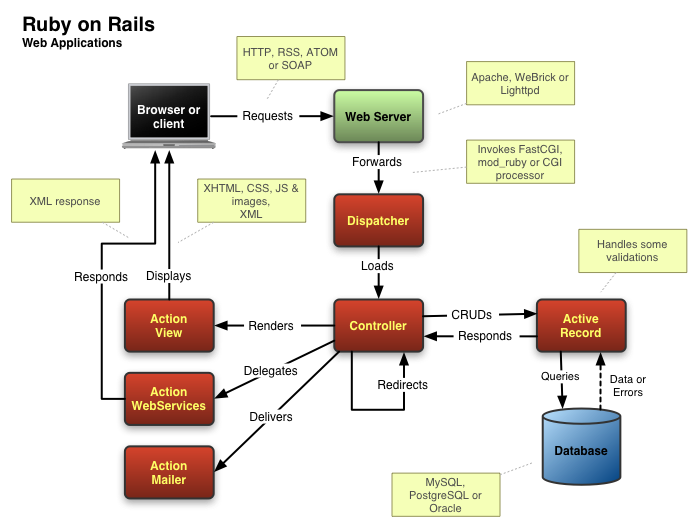
\includegraphics[width=0.7\textwidth]{images/figures/rubyonrails.png}
\caption{Integración entre características y componentes de Ruby on Rails.\label{fig:figure_placement_example}}
\end{figure}

Una vez vistas las características y capacidades, tanto de una aplicación Ruby on Rails genérica como de la aplicación en actual estudio, se decide elaborar un trabajo adicional sobre ella, aplicando una serie de cambios y adiciones para la consecusión de los objetivos propuestos, inicialmente.

\section{Iteración 1: Conversión de una aplicación Ruby on Rails a una arquitectura de microservicios}

La primera iteración del proyecto consiste en adecuar la aplicación Ruby on Rails para que utilice contenedores en su funcionamiento. Esta tarea supone su despliegue en una sola máquina física.

La aplicación \kode{sample\_app\_rails\_4} está disponible en un repositorio GitHub. Para trabajar con ella se hace una copia del repositorio a través de un \textit{fork}. Esto crea una bifurcación que permite la libre experimentación de cambios, sin afectar el proyecto original, utilizando el proyecto de otra persona como punto de partida de una idea propia.

Una vez se tiene una copia local y se comprueba que funciona correctamente se va a hacer uso de la tecnología de contenerización Docker para desplegar la siguiente estructura:

\begin{figure}[H]
\image{images/figures/iteration1.png}
\caption{Estructura del despliegue monomáquina con contenedores Docker.\label{fig:figure_docker_microservices}}
\end{figure}

Mediante Docker se obtienen las imágenes pertenecientes a dos servicios. El primero implementa la funcionalidad de la base de datos \kode{PostgreSQL} y el segundo implementa el servidor web y proxy inverso \kode{Nginx}. El proxy inverso es un proxy que aparenta ser un servidor web ante los clientes, pero que en realidad reenvía las solicitudes que recibe a uno o más servidores de origen. Se escoge \kode{Nginx} por ser multiplataforma, ligero, de alto rendimiento y software libre.

La aplicación en su origen utiliza una base de datos \kode{SQLite}\footnotettt{SQLite}{https://sqlite.org} que va a ser cambiada por la base de datos \kode{PostgreSQL}, provisionada por el contenedor \kode{some-postgres}. 

Otro de los cambios a implementar es la sustitución del servidor web \kode{rails s} por \kode{puma}\footnotettt{Servidor Web Puma}{http://puma.io}, construido para ofrecer mayor velocidad y paralelismo.

Como se ha comentado, a través de Docker se pueden obtener las imágenes de los servidores \kode{PostgreSQL} y \kode{Nginx}, pero para poder crear un contenedor que contenga la aplicación web habrá que crear su imagen Docker. 

El principal propósito de este despliegue es que pueda realizarse automáticamente tras la ejecución de un \textit{script}. Este fichero comprobará que las variables de entorno que especifican el nombre y la contraseña del usuario de las distintas bases de datos PostgreSQL existentes (test, desarrollo y producción) están correctamente establecidas.

La siguiente acción a realizar será la construcción de la imagen Docker de la aplicación web, que se llamará \kode{sample\_app\_rails\_4\_image}. 

Luego se creará el contenedor \kode{some-postgres} con el servidor \kode{PostgreSQL} y, seguidamente, se creará el contenedor de la aplicación web, llamado \kode{some-app}, a partir de la imagen de ésta, enlazándola con el contenedor \kode{some-postgres}, que será su base de datos.

Con la intención de utilizar como servidor web de la aplicación un contenedor diferente al propio, se crea el contenedor \kode{some-nginx} que proporciona el servidor \kode{Nginx}. Se le indicará que el tráfico del puerto 8080 en el sistema anfitrión se redirija al 80 del contenedor. Así, el sitio web será accesible por la dirección local en el puerto 8080. Además, se enlazará a la aplicación web mediante el contenedor en el que se ejecuta, y se montará el volumen Docker compartido \kode{volume-public}.

Así, solo quedará construir, migrar y poblar la base de datos que se ejecuta en el contenedor \kode{some-app}, dentro del contenedor \kode{some-postgres}.

Finalmente, se ejecutará el servidor \kode{puma} dentro del contenedor \kode{some-app} y se comprobará desde el sistema anfitrión que la página principal de la aplicación \kode{sample\_app\_rails\_4} está disponible en el puerto 8080. Esto producirá el siguiente resultado:

\begin{figure}[H]
\centering
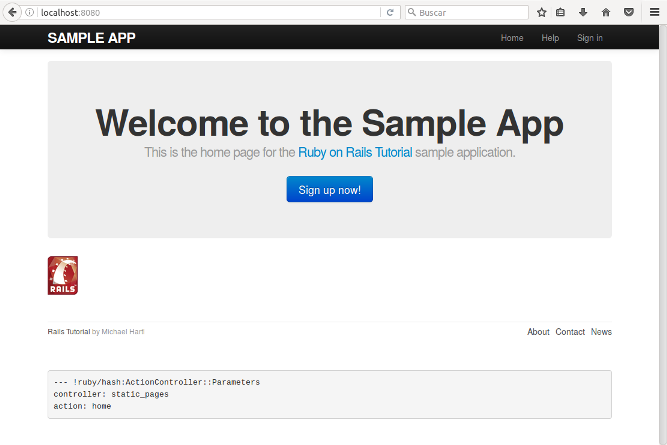
\includegraphics[width=0.8\textwidth]{images/figures/resultado1.png}
\caption{Resultado de la Iteración 1 con el uso de Docker.\label{fig:figure_placement_example}}
\end{figure}

A efectos de mantener la imagen de la aplicación remotamente se subirá al repositorio DockerHub con la etiqueta \kode{initial}.

\subsection{Preparación del repositorio local y remoto}

En primer lugar se realiza una copia del repositorio GitHub de la aplicación \kode{sample\_app\_rails\_4}. Para ello se realiza un \textit{fork} seleccionando el botón con el mismo nombre y automáticamente se crea la copia del repositorio en la cuenta personal. Seguidamente se clona esta copia para trabajar localmente:

%= lang:bash
\begin{code}
$ git clone https://github.com/CarolinaSantana/sample_app_rails_4-1.git 
\end{code}

Luego se entra en la carpeta local que lo contiene, seleccionando como \textit{gemset}, conjunto aislado de gemas incorporadas en la aplicación para la versión Ruby en uso, 2.0.0, quedando como \kode{2.0.0@railstutorial\_rails\_4\_0}. Además se deja lista la configuración de base de datos, utilizando la que viene a modo de ejemplo, con la intención de probar que los test que comprueban su funcionalidad pasen positivamente: 

%= lang:bash
\begin{code}
$ cd sample_app_rails_4-1
$ cp config/database.yml.example config/database.yml
$ bundle install --without production
$ bundle exec rake db:migrate
$ bundle exec rake db:test:prepare
$ bundle exec rspec spec/
\end{code}

\subsection{Cambio y configuración de la base de datos} \label{postgrescredentials}

Una vez completada la fase de preparación de la aplicación en el entorno local se quiere desplegar la estructura definida en la Figura \ref{figure_docker_microservices}, página \pageref{figure_docker_microservices}.

Con la intención de implementar la base de datos de la aplicación desde un contenedor Docker se elimina del fichero \kode{Gemfile} la gema \kode{sqlite3 1.3.8}, como base de datos en desarrollo, y se cambia por una base de datos PosgreSQL, concretamente la versión \kode{pg 0.15.1}. Para instalar la nueva gema se ejecuta:

%= lang:bash
\begin{code}
$ bundle install --without production
\end{code}

La instalación de \kode{PostgreSQL} requiere credenciales de usuario con contraseña para acceder. La manera de especificarlo es mediante las variables de entorno \kode{\$POSTGRES\_USER} y \kode{\$POSTGRES\_PASSWORD} en el fichero local \kode{\textasciitilde{}/.postgres/credentials} cuyo contenido es:

\begin{codelisting}
\label{code:credentials}
\codecaption{Fichero \kode{\textasciitilde{}/.postgres/credentials}}
\begin{code}
export POSTGRES_USER=postgres
export POSTGRES_PASSWORD=postgres
\end{code}
\end{codelisting}

Se da permiso de ejecución tanto al fichero como a la carpeta que lo contiene y se exportan las variables de entorno en el directorio de la aplicación:

%= lang:bash
\begin{code}
$ chmod 0700 ~/.postgres
$ chmod 0700 ~/.postgres/credentials
$ . ~/.postgres/credentials
\end{code}

Ahora hay que cambiar el fichero de configuración de la base de datos de forma que se especifique lo siguiente:

\begin{codelisting}
\label{code:database}
\codecaption{Cambios en el fichero \kode{config/database.yml}}
\begin{code}
default: &default
  adapter: postgresql
  encoding: unicode
  pool: 5
  username: <%= ENV['POSTGRES_USER'] %>
  password: <%= ENV['POSTGRES_PASSWORD'] %>
  port: 5432

development:
  <<: *default
  database: sample_app_development  
  host : db

test:
  <<: *default
  database: sample_app_test
  host: db

production:
  <<: *default
  database: sample_app_production
\end{code}
\end{codelisting}

De esta manera se ha indicado a las bases de datos de desarrollo, test y producción el nombre de usuario y contraseña, que capturará a partir de las variables de entorno, y que ha de conectarse a \textit{db}, que será el nombre por el que ha de descubrir el contenedor docker que provisiona el servidor \kode{PostgreSQL}.

Por motivos de seguridad el fichero de configuración de la base de datos no se ha de subir al repositorio remoto, por lo que se hace una copia para tener esta configuración de ejemplo:

%= lang:bash
\begin{code}
$ cp config/database.yml config/database.yml.postgres
\end{code}

\subsection{Creación de un alimentador de base de datos idempotente}

Con la intención de que cuando ya existan datos en la base de datos no se vuelvan a crear, se cambia el fichero \kode{lib/tasks/sample\_data.rake}, que viene por defecto, para que sea un \textit{seed} idempotente. Solo se crearán datos en la base de datos si aún no existen, quedando el fichero como:

\begin{codelisting}
\label{code:idempotentseed}
\codecaption{Fichero \kode{lib/tasks/sample\_data.rake}}
%= lang:ruby
\begin{code}
namespace :db do
  desc "Fill database with sample data"
  task populate: :environment do
    make_users_microposts_relationships
  end
end

def make_users_microposts_relationships
  User.find_or_create_by(email:"example@railstutorial.org") do |admin| 
  	admin.name = "Example User"
	admin.password = "foobar"
        admin.password_confirmation = "foobar"
        admin.admin = true

	99.times do |n|
	    name  = Faker::Name.name
	    email = "example-#{n+1}@railstutorial.org"
	    password  = "password"
	    User.create!(name:     name,
                 email:    email,
                 password: password,
                 password_confirmation: password)
        end

	users = User.all(limit: 6)
  	50.times do
	    content = Faker::Lorem.sentence(5)
	    users.each { |user| user.microposts.create!(content: content) }
	end  

	users = User.all
	user  = users.first
	followed_users = users[2..50]
	followers      = users[3..40]
	followed_users.each { |followed| user.follow!(followed) }
	followers.each      { |follower| follower.follow!(user) }
  end
end
\end{code}
\end{codelisting}

\subsection{Cambio y configuración del servidor web}

Por su parte, para poder acceder a la aplicación en cuestión, se cambia el servidor web \kode{rails s} por \kode{puma}\footnotettt{Servidor Web Puma}{http://puma.io}. Para ello se añade al fichero \kode{Gemfile} la siguiente entrada:

\begin{codelisting}
\label{code:addpuma}
\codecaption{Fichero \kode{Gemfile}}
%= lang:ruby
\begin{code}
.
gem 'puma'
.
\end{code}
\end{codelisting}

Luego se instala la nueva gema: 

%= lang:bash
\begin{code}
$ bundle install --without production
\end{code}

\subsection{Configuración automatizada para la creación de los contenedores}

En primer lugar se configuran los registros o \textit{logs} que crearán los contenedores añadiendo en el fichero \kode{config/application.rb} lo siguiente:

\begin{codelisting}
\label{code:application.rb}
\codecaption{Fichero \kode{config/application.rb}}
%= lang:ruby
\begin{code}
.
config.logger = Logger.new(STDOUT)
.
\end{code}
\end{codelisting}

Además, se añade el fichero \kode{.dockerignore} para que la imagen Docker del repositorio que se construya sea más ligera:

\begin{codelisting}
\label{code:.dockerignore}
\codecaption{Fichero \kode{.dockerignore}}
%= lang:ruby
\begin{code}
.
cp .gitignore .dockerignore
.
\end{code}
\end{codelisting}

En este momento ya se tienen listas las configuraciones necesarias para proceder a la creación de los contenedores. Para ello se comienza a ejecutar el script \kode{docker-microservice.sh}.

En primer lugar, se comprueba que las variables de entorno que especifican el nombre y la contraseña del usuario de la base de datos PostgreSQL están establecidas.

Para crear el contenedor de la aplicación primero se construye su imagen, que se llamará \kode{sample\_app\_rails\_4\_image}. Así, es necesario crear un fichero \kode{Dockerfile} que especifica cómo crearla, indicando que lo hará a partir de una imagen Ruby y que debe actualizar todos los paquetes e instalar \textit{nodejs}, requerido por la aplicación, y la utilidad netcat, para comprobar que el servicio PostgreSQL está listo. Tras ello se le indica que haga una limpieza de las capas intermedias. 

La lógica de construcción de la aplicación basada en su imagen pasa por la creación de dos contenedores. El primer contenedor, \kode{app-job}, se configurará a partir de un \textit{entrypoint} que permite ejecutar un contenedor como un ejecutable. Este contenedor esperará a que el servicio \textit{PostgreSQL} esté activo en el contenedor \kode{some-postgres} para crear, migrar, alimentar y poblar las bases de datos. Una vez acaba el contenedor también termina. Para poder especificar el \textit{entrypoint} es necesario copiar el fichero script \kode{setup.sh}, que se encarga de ello, dentro del contenedor, indicando la copia en \kode{Dockerfile}. 

\begin{codelisting}
\label{code:dockerfile}
\codecaption{Fichero \kode{setup.sh}}
%= lang:ruby
\begin{code}
#!/bin/sh

cp config/database.yml.postgresql config/database.yml

echo "Waiting PostgreSQL to start on 5432..."

while ! nc -z some-postgres 5432; do
  sleep 0.1
done

echo "PostgreSQL started"

echo "Creating databases..."
rake db:create

echo "Migrating to databases..."
rake db:migrate

echo "Seeding databases..."
rake db:seed

echo "Populating databases..."
rake db:populate

echo "Ready databases"

\end{code}
\end{codelisting}

Así como se tiene el contenedor \textit{job} se necesita un segundo contenedor \textit{task}, concretamente llamado \kode{app-task}. Este contenedor se construye a partir del anterior.

\begin{codelisting}
\label{code:dockerfile}
\codecaption{Contenido de \kode{Dockerfile}}
%= lang:ruby
\begin{code}
##################################################
# Dockerfile to build a sample_app_rails_4 image #
# Version 0.1                                    #
##################################################
FROM ruby:2.0-onbuild
LABEL sample_app_rails_4_image.version="0.1" 
      sample_app_rails_4_image.release-date="2016-12-10"
MAINTAINER Carolina Santana "c.santanamartel@gmail.com"
RUN apt-get update && apt-get -y install nodejs && \
    apt-get -y install netcat && \
    apt-get autoclean && apt-get clean && \
    rm -rf /var/lib/apt/lists/* && \
    rm -f /tmp/* /var/tmp/*
COPY /setup.sh /
\end{code}
\end{codelisting}

La siguiente acción es la creación del contenedor \kode{some-postgres} con el servidor \kode{PostgreSQL}, a partir de la imagen \kode{postgres} indicada con \textit{\--d}. Para poder acceder a la base de datos es necesario pasarle las credenciales, con \textit{\--e}. 

Con la intención de exportar un volumen compartido entre los contenedores \kode{app-task} y \kode{some-nginx} para que compartan el directorio \kode{/usr/src/app/public} se crea un volumen Docker llamado \kode{volume-public}.

Ahora se crea el contenedor \textit{job} de la aplicación web, llamado \kode{app-job}, a partir de la imagen de ésta, \textit{\--d}, indicando como \textit{\---entrypoint} el script comentado, enlazando la base de datos de la misma con el contenedor \kode{some-postgres} a través del indicador \textit{\--link}. Además, se le pasan las variables de entorno necesarias para acceder a la base de datos, con \textit{\--e}. Por su parte, el indicador \textit{\--it} ofrece un terminal interactivo dentro del contedor y \textit{\--w} indica que se va a compartir el directorio inicial del proyecto local en el contenedor. El volumen creado se exporta mediante \textit{\--v}.

El siguiente paso crea el contenedor \textit{task} de la aplicación web, llamado \kode{app-task}. Este se construye como el anterior obviando el paso del \textit{entrypoint}. Además, se configuran y preparan las bases de datos, así como se ejecuta el servidor \kode{puma} en el puerto \kode{9292} para que la aplicación pueda ser accesible, todo ello a través de \textit{/bin/bash \--c}

Para crear el contenedor \kode{some-nginx} que proporciona el servidor \kode{Nginx} se indica la imagen con \textit{\--d}, que el tráfico del puerto 8080 en el sistema anfitrión se redirija al 80 del contenedor, \textit{\--p}, y se enlaza la aplicación web con el contenedor en el que se ejecuta, a través del indicador \textit{\--link}. Además se monta el volumen \kode{volume-public} con el indicador \textit{\--v}. Por último, se crea localmente el fichero de configuración \kode{/etc/nginx/conf.d/nginx.conf} en el que se especifica que este servidor escuchará en el puerto 80, compartiendo el directorio \kode{/usr/src/app/public}, también indicado en la creación con \textit{\--w}, así como que ha de resolver la aplicación en el puerto 9292, que es el que usa \kode{puma} para la ejecución.  

El contenido de este fichero es: 
\begin{codelisting}
\label{code:nginxconf}
\codecaption{Contenido de \kode{nginx.conf}}
%= lang:java
\begin{code}
server {
  listen 80;

  root /usr/src/app/public;
  location / {
    proxy_set_header X-Forwarded-For $proxy_add_x_forwarded_for;
    proxy_set_header Host $http_host;
    proxy_redirect off;
    try_files $uri /page_cache/$uri /page_cache/$uri.html @app;
  }
  
  location @app{
    proxy_pass http://app:9292;
    break;
  }
}
\end{code}
\end{codelisting}

Así, se accede al contenedor \kode{some-app} para poder construir, migrar y poblar la base de datos que se ejecuta en el contenedor \kode{some-app}, dentro del contenedor \kode{some-postgres}.

El script utilizado, con permiso \kode{chmod +x} y ejecutado como \kode{./docker-microservices.sh}, es el siguiente:

\begin{codelisting}
\label{code:scriptdocker}
\codecaption{Contenido de \kode{docker-microservices.sh}}
%= lang:bash
\begin{code}
#!/bin/bash

if [ "$POSTGRES_USER" = "" ] || [ "$POSTGRES_PASSWORD" = "" ]; then
	echo "Environment variables for POSTGRES not found"
        exit
fi

docker build -t sample_app_rails_4_image .

docker run --name some-postgres -e POSTGRES_USER=$POSTGRES_USER \
  -e POSTGRES_PASSWORD=$POSTGRES_PASSWORD -d postgres

docker volume create --name volume-public

docker run -i --name app-job --entrypoint /setup.sh \
  -e POSTGRES_USER=$POSTGRES_USER -e POSTGRES_PASSWORD=$POSTGRES_PASSWORD \
  -w /usr/src/app -v volume-public:/usr/src/app/public \
  --link some-postgres:db sample_app_rails_4_image

docker run -d -it --name app-task -e POSTGRES_USER=$POSTGRES_USER \
  -e POSTGRES_PASSWORD=$POSTGRES_PASSWORD -w /usr/src/app \
  -v volume-public:/usr/src/app/public --link some-postgres:db \
  sample_app_rails_4_image \
  /bin/bash -c "cp config/database.yml.postgresql config/database.yml && puma -p 9292"

docker run --name some-nginx \
  -v "${PWD}/nginx.conf":/etc/nginx/conf.d/default.conf \
  -p 8080:80 --link app-task:app -v volume-public:/usr/src/app/public -d nginx
\end{code}
\end{codelisting}

\subsection{Resultado}

El resultado del script anterior crea los distintos elementos propuestos en el planteamiento de esta iteración. Así las imagenes Docker descargadas y la creada, perteneciente a la aplicación, son:

\begin{figure}[H]
\centering
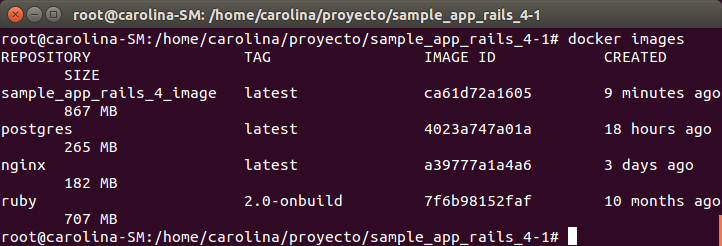
\includegraphics[width=0.8\textwidth]{images/figures/dockerimages.png}
\caption{Imágenes docker mostradas con \kode{docker images}.\label{fig:figure_placement_example}}
\end{figure}

Y los contenedores Docker creados son:

\begin{figure}[H]
\centering
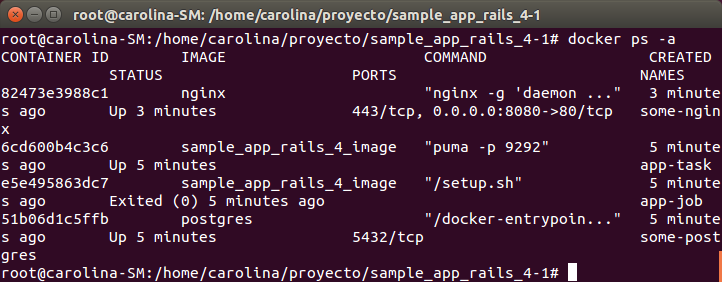
\includegraphics[width=0.8\textwidth]{images/figures/dockerps.png}
\caption{Contenedores docker mostrados con \kode{docker ps -a}.\label{fig:figure_placement_example}}
\end{figure}

De esta manera, en el contenedor \kode{app-task} se encuentra en ejecución el servidor \kode{puma}, así que se puede comprobar desde el sistema anfitrión que la página principal de la aplicación \kode{sample\_app\_rails\_4} está disponible en el puerto 8080, mediante el comando \kode{curl http://localhost:8080}:

\begin{figure}[H]
\centering
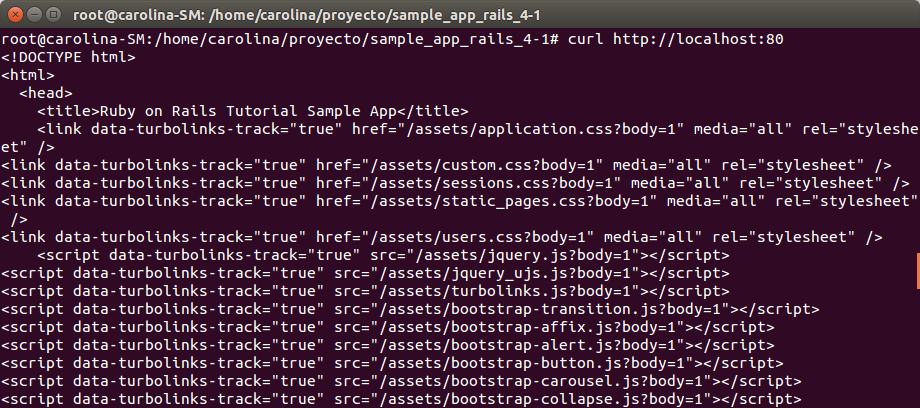
\includegraphics[width=0.8\textwidth]{images/figures/curldocker.png}
\caption{Volcado de ejecución \kode{curl http://localhost:8080}.\label{fig:figure_placement_example}}
\end{figure}

Así, a partir de ahora se podrá hacer el despliegue partiendo de la imagen local. Para poder hacerlo de forma automatizada se crea el fichero \kode{docker-microservices-deploy.sh}, con permiso \kode{chmod +x} y ejecutado como \kode{./docker-microservices.sh}, es el siguiente:

\begin{codelisting}
\label{code:scriptdocker}
\codecaption{Contenido de \kode{docker-microservices-deploy.sh}}
\begin{code}
#!/bin/bash

if [ "$POSTGRES_USER" = "" ] || [ "$POSTGRES_PASSWORD" = "" ]; then
	echo "Environment variables for POSTGRES not found"
        exit
fi

docker run --name some-postgres -e POSTGRES_USER=$POSTGRES_USER \
  -e POSTGRES_PASSWORD=$POSTGRES_PASSWORD -d postgres

docker volume create --name volume-public

docker run -i --name app-job --entrypoint /setup.sh -e POSTGRES_USER=$POSTGRES_USER \
  -e POSTGRES_PASSWORD=$POSTGRES_PASSWORD -w /usr/src/app \
  -v volume-public:/usr/src/app/public --link some-postgres:db \
  carolina/sample_app_rails_4_image:latest

docker run -d -it --name app-task -e POSTGRES_USER=$POSTGRES_USER \
  -e POSTGRES_PASSWORD=$POSTGRES_PASSWORD -w /usr/src/app \
  -v volume-public:/usr/src/app/public --link some-postgres:db \
  carolina/sample_app_rails_4_image:latest \
  /bin/bash -c "cp config/database.yml.postgresql config/database.yml && puma -p 9292"

docker run --name some-nginx -v "${PWD}/nginx.conf":/etc/nginx/conf.d/default.conf \
  -p 8080:80 --link app-task:app -v volume-public:/usr/src/app/public -d nginx
\end{code}
\end{codelisting}

De esta forma, este despliegue operará y ofrecerá los servicios de la misma manera que el anterior.

\section{Iteración 2: Subida de la imagen a DockerHub}

A efectos de mantener la imagen remotamente se sube al repositorio DockerHub, previa creación de una cuenta en él. Para ello se inicia sesión por consola y se añade una etiqueta a la imagen \kode{sample\_app\_rails\_4\_image}, especificando su identificador y el repositorio escogido dentro de la cuenta:

%= lang:bash
\begin{code}
$ docker login
$ docker tag <image-id> carolina/sample_app_rails_4_image:initial
$ sudo docker push carolina/sample_app_rails_4_image
\end{code}

Cuando se muestran las imágenes docker se aprecia la etiquetación hecha:

\begin{figure}[H]
\centering
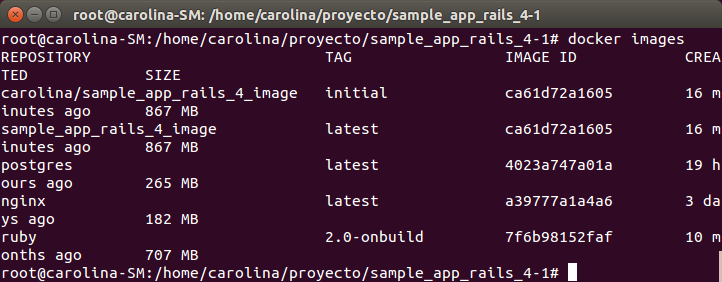
\includegraphics[width=0.8\textwidth]{images/figures/dockerimages2.png}
\caption{Imágenes docker mostradas con \kode{docker images}.\label{fig:figure_placement_example}}
\end{figure}

La subida de la imagen etiquetada como \kode{initial} se puede apreciar ahora en Docker Hub:

\begin{figure}[H]
\centering
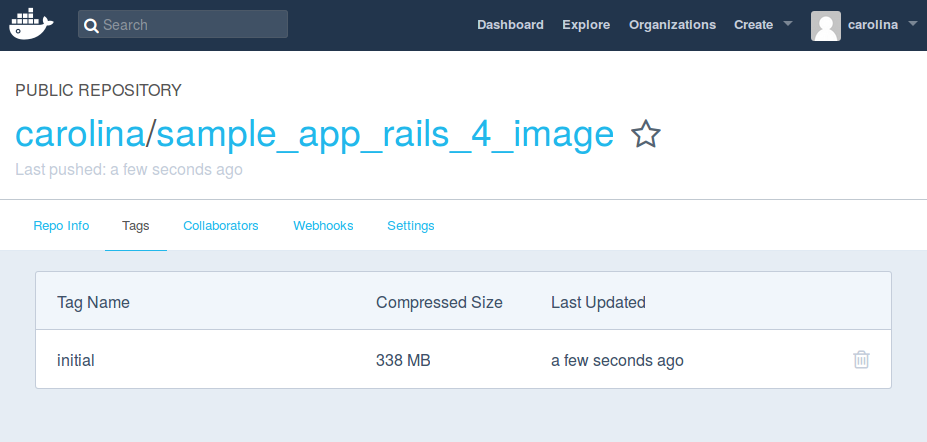
\includegraphics[width=0.8\textwidth]{images/figures/dockerhubinitial.png}
\caption{Imágenes docker mostradas con \kode{docker images}.\label{fig:figure_placement_example}}
\end{figure}

También puede ser comprobado localmente mediante:

%= lang:bash
\begin{code}
$ docker 
$ docker tag <image-id> carolina/sample_app_rails_4_image:initial
$ sudo docker push carolina/sample_app_rails_4_image
\end{code}

Cuyo resultado es:

\begin{figure}[H]
\image{images/figures/dockerimages3.png}
\caption{Resultado de la búsqueda de la imagen con \kode{docker search}.\label{fig:figure_placement_example}}
\end{figure}

\section{Iteración 3: Integración y Despliegue continuos con Travis CI}

En esta iteración se busca adaptar la aplicación Ruby on Rails para que funcione con Travis CI. Esta herramienta se conectará al repositorio de GitHub \kode{sample\_app\_rails\_4-1} con la intención de poder generar una imagen Docker de la aplicación tras cada cambio. Esto permite trabajar en un entorno de desarrollo en el que la integración de los cambios en el proyecto es continua, así como también su despliegue es automatizado.

Para ello se realiza el siguiente proceso:
\begin{figure}[H]
\image{images/figures/iteration2.png}
\caption{Integración y Despliegue continuos con Travis CI.\label{fig:figure_placement_example}}
\end{figure}

Las precondiciones, condiciones y postcondiciones necesarias para construir y desplegar la aplicación en uso de manera automática se especifican en el fichero \kode{.travis.yml}. A este fichero se le añadirán, además, las credenciales de la cuenta de DockerHub mediante variables de entorno encriptadas, sumando una respectiva al repositorio GitHub. Las acciones a realizar serán la comprobación de que los tests pasan satisfactoriamente, la construcción de una nueva imagen Docker y su subida al repositorio DockerHub.

Para llevarlo a cabo es necesario añadir una configuración de base de datos específica. En este caso se llamará \kode{travis\_ci\_test}.

Finalmente, el resultado permitirá que cuando se haga un nuevo cambio o \textit{commit} acompañado de una subida del mismo al repositorio GitHub comenzará, también, la construcción en Travis CI. Tanto en caso de fallo como de éxito se configura el envío de un correo electrónico que lo anuncie. Al repositorio en DockerHub se subirán 3 copias comprimidas de la imagen. La primera etiquetada con el hash del \textit{commit}, la segunda con el número de construcción en Travis CI y la tercera como la última versión, \textit{latest}:

\begin{figure}[H]
\centering
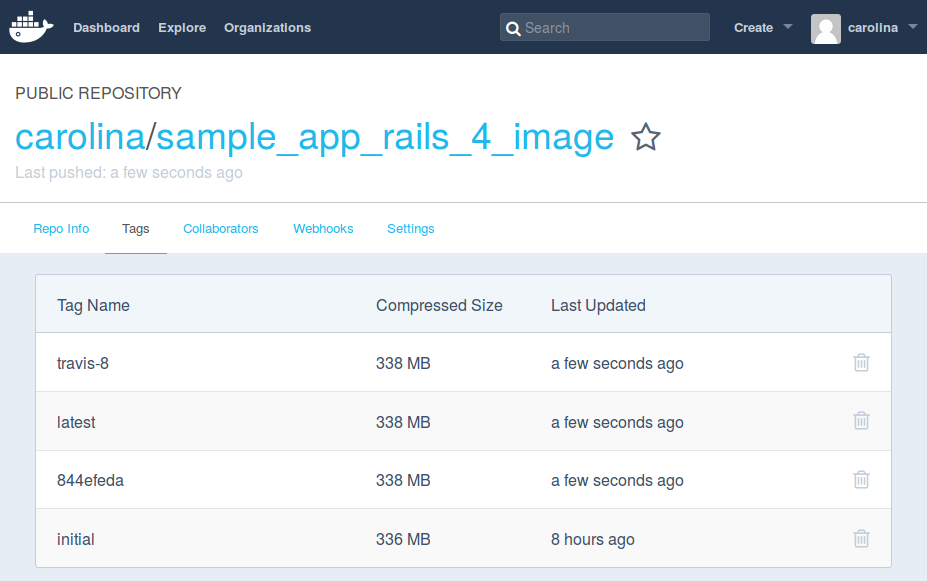
\includegraphics[width=0.8\textwidth]{images/figures/dockerhubimages.png}
\caption{Repositorio de \kode{sample\_app\_rails\_4\_image}.\label{fig:dockerhub_images}}
\end{figure}

\subsection{Vinculación con el repositorio remoto}

En primer lugar hay que ingresar en el sitio Travis CI con la cuenta de GitHub y añadir el repositorio con el que se trabaja actualmente:

\begin{figure}[H]
\image{images/figures/travis_github.png}
\caption{Vinculación de GitHub con Travis CI.\label{fig:travis_github}}
\end{figure}

\subsection{Configuración y establecimiento de precondiciones, condiciones y postcondiciones}

En segundo lugar se procede a instalar la nueva gema. Para ello se edita el fichero \kode{Gemfile}, incluyendo:

\begin{codelisting}
\label{code:addtravis}
\codecaption{Fichero \kode{Gemfile}}
%= lang:ruby
\begin{code}
.
group :development, :test do
  gem 'travis'
.
end
.
\end{code}
\end{codelisting} 

Luego se instala mediante:

%= lang:bash
\begin{code}
$ bundle install --without production
\end{code}

Una vez instalada, es necesario crear un nuevo fichero de configuración para la base de datos en Travis CI, que permitirá probar el correcto funcionamiento:
\begin{codelisting}
\label{code:travisdatabase}
\codecaption{Fichero \kode{config/database.yml.travis} }
%= lang:ruby
\begin{code}
test:
  adapter: postgresql
  database: travis_ci_test
  username: postgres
\end{code}
\end{codelisting}

Para configurar Travis CI se crea el fichero \kode{.travis.yml}. 

%= lang:bash
\begin{code}
$ touch .travis.yml
\end{code}

Tras ello, hay que establecer las variables de entorno correspondientes a las credenciales de DockerHub. Esto se especifica localmente mediante la ejecución de los siguientes comandos:

%= lang:bash
\begin{code}
$ travis env set DOCKER_USERNAME carolina
$ travis env set DOCKER_PASSWORD **************
\end{code}

También se agrega una variable de entorno que contenga los 8 primeros caracteres del \textit{hash} del \textit{git commit}, justo debajo de las anteriores.

En la sección \kode{after\_success} del fichero se inicia sesión en DockerHub y luego se construye la imagen. Al repositorio en DockerHub se subirán 3 copias comprimidas de la imagen. La primera etiquetada con el hash del \textit{commit} correspondiente, la segunda con el número de construcción en Travis CI y la tercera como la última versión, \textit{latest}. Además se le indica la base de datos de prueba para la ejecución de los tests y la versión de Ruby en uso.

El fichero definido queda de la siguiente forma:

\begin{codelisting}
\label{code:travis}
\codecaption{Fichero \kode{.travis.yml} }
%= lang:ruby
\begin{code}
env:
  global:
  - COMMIT=${TRAVIS_COMMIT::8}
language: ruby
rvm:
- 2.0.0-p648
bundler_args: --without production
addons:
  postgresql: '9.3'
services:
- docker
before_script:
- cp config/database.yml.travis config/database.yml
- psql -c 'create database travis_ci_test;' -U postgres
- RAILS_ENV=test bundle exec rake db:migrate --trace
script:
- bundle exec rspec
notifications:
  email:
    recipients:
    - c.santanamartel@gmail.com
    on_success: always
    on_failure: always
sudo: required
after_success:
- docker login -u $DOCKER_USERNAME -p $DOCKER_PASSWORD
- export REPO=$DOCKER_USERNAME/sample_app_rails_4_image
- docker build -f Dockerfile -t $REPO:$COMMIT .
- docker tag $REPO:$COMMIT $REPO:latest
- docker tag $REPO:$COMMIT $REPO:travis-$TRAVIS_BUILD_NUMBER
- docker push $REPO  
\end{code}
\end{codelisting}

Con la intención de compartir el repositorio GitHub con la comunidad, se crea una copia donde se borran manualmente las credenciales \kode{secure} para no exponerlas ya que, aunque esten encriptadas, si otro usuario hiciera uso del repositorio podría realizar nuevas subidas de imágenes en él, 
%= lang:bash
\begin{code}
$ cp .travis.yml .travis.yml.sample
\end{code}

Además se oculta el fichero \kode{.travis.yml} en GitHub y DockerHub:

\begin{codelisting}
\label{code:scriptdocker}
\codecaption{Añadido a los ficheros \kode{.gitignore} y \kode{.dockerignore}}
%= lang:bash
\begin{code}
.
.travis.yml
.
\end{code}
\end{codelisting}

\subsection{Resultado}

Finalmente, cuando se haga un nuevo \textit{commit} y subida al repositorio GitHub comenzará también la construcción en Travis CI. Tanto si se produce un fallo como si termina con éxito se ha configurado el envío de un correo electrónico para informarlo. Así, el caso de fallo se prueba comentando la línea que crea la base de datos de prueba \kode{travis\_ci\_test} y el de éxito con ella. De esta manera, los correos electrónicos recibidos son:

\begin{figure}[H]
\centering
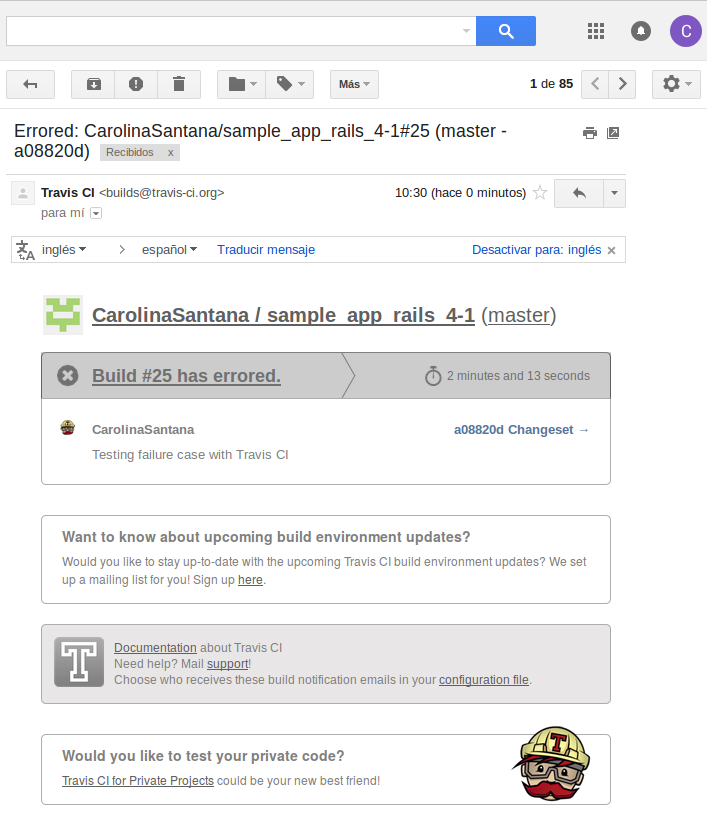
\includegraphics[width=0.7\textwidth]{images/figures/travisfailure.png}
\caption{Correo electrónico de Travis CI en caso de fallo.\label{fig:figure_placement_example}}
\end{figure}

\begin{figure}[H]
\centering
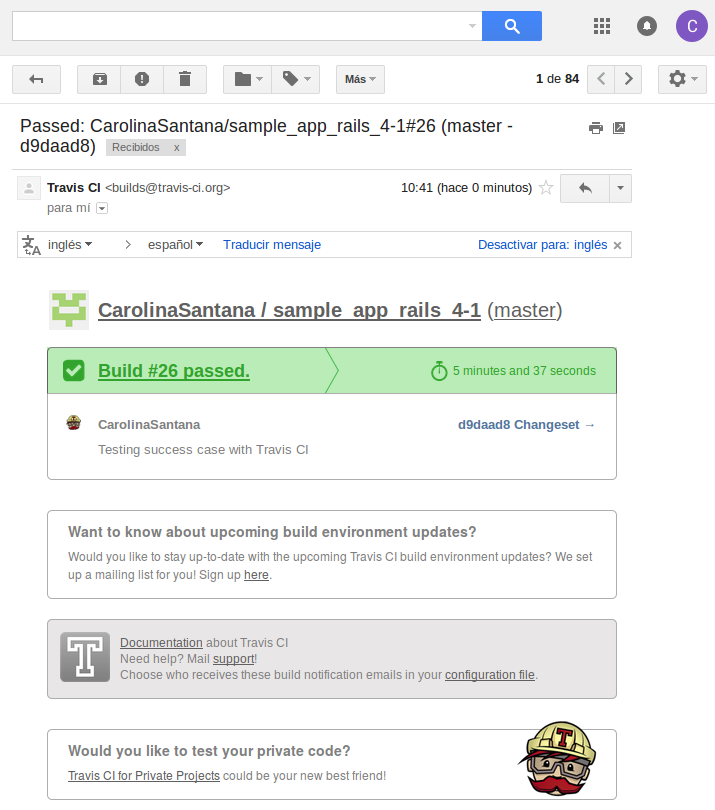
\includegraphics[width=0.7\textwidth]{images/figures/travissuccess.png}
\caption{Correo electrónico de Travis CI en caso de éxito.\label{fig:figure_placement_example}}
\end{figure}

Dirigiendo a Travis CI donde se comenta el fallo o el éxito:

\begin{figure}[H]
\centering
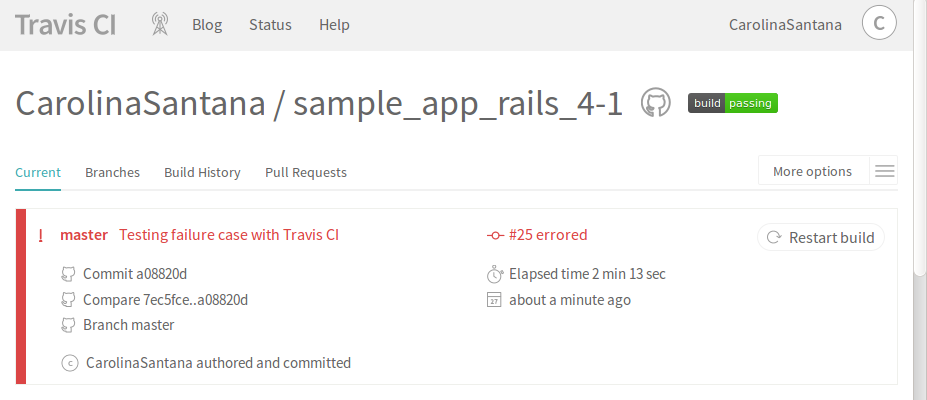
\includegraphics[width=0.8\textwidth]{images/figures/travisfailure2.png}
\caption{Caso de fallo en Travis CI.\label{fig:figure_placement_example}}
\end{figure}

\begin{figure}[H]
\centering
\image{images/figures/travisfailure3.png}
\caption{Motivo de fallo en Travis CI.\label{fig:figure_placement_example}}
\end{figure}

\begin{figure}[H]
\centering
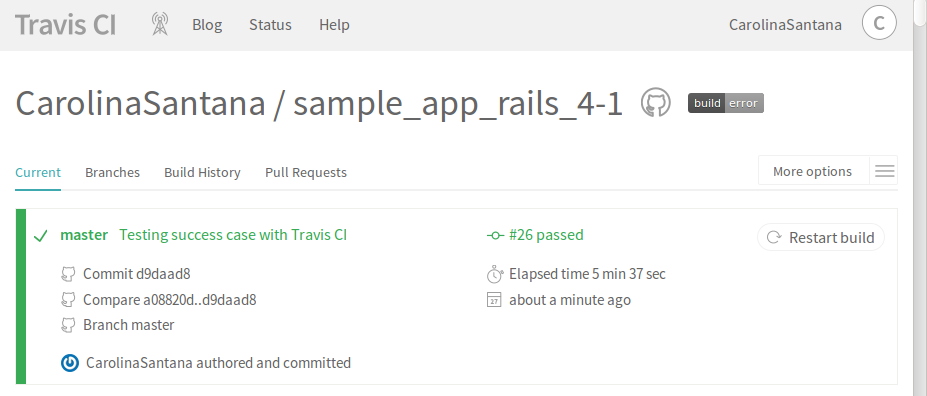
\includegraphics[width=0.8\textwidth]{images/figures/travissuccess2.png}
\caption{Caso de éxito en Travis CI.\label{fig:figure_placement_example}}
\end{figure}

Esta construcción terminará con la creación y subida de las tres imágenes comentadas en el planteamiento de esta iteración \ref{fig:dockerhub_images} en el repositorio de DockerHub.

\section{Iteración 4: Despliegue monomáquina con unidades de servicio usando CoreOS}

En esta nueva iteración se quiere aplicar el uso del sistema operativo orientado a contenedores CoreOS. De esta manera se crearán unidades de servicio \kode{systemd} que se encargarán de realizar las tareas necesarias para la correcta aplicación y funcionamiento de los contenedores Docker en los que se divide la aplicación. Así, el nuevo planteamiento es el siguiente:

\begin{figure}[H]
\centering
\image{images/figures/coreosdiagram.png}
\caption{Estructura del despliegue monomáquina con unidades de servicio CoreOS.\label{fig:figure_placement_example}}
\end{figure}

De esta manera se puede observar como en local existen dos herramientas de línea de comandos llamadas \kode{fleectl} y \kode{etcdctl} utilizadas internamente para comunicarse con los elementos del sistema CoreOS \kode{fleetd} y \kode{etcd}. Fleet se encarga de dotar a la máquina CoreOS los servicios que se desean implementar. Etcd permite almacenar las estructuras y datos pertinentes en la máquina CoreOS.

\subsection{Preparación del repositorio local y remoto}

En primer lugar se realiza una copia del repositorio GitHub \kode{CoreOS Vagrant} que proporciona una plantilla \kode{Vagrantfile} para configurar el entorno de una máquina virtual CoreOS, usando el hipervisor software VirtualBox. 

Una vez finalizada la instalación, se tendrá una única máquina virtual CoreOS que se ejecutará localmente. Para ello se realiza un \textit{fork} seleccionando el botón con el mismo nombre y automáticamente se crea la copia del repositorio en la cuenta personal. Seguidamente se clona esta copia para trabajar localmente:

%= lang:bash
\begin{code}
$ git clone https://github.com/CarolinaSantana/coreos-vagrant.git 
\end{code}

Luego, se accede a la carpeta local que lo contiene y se prepara para comprobar su funcionamiento con los datos de usuario y la configuración de ejemplo. Esto se prueba ejecutando el \kode{Vagrantfile} y conectándose a la máquina virtual creada: 

%= lang:bash
\begin{code}
$ cd coreos-vagrant
$ cp user-data.sample user-data
$ cp config.rb.sample config.rb
$ vagrant up
$ vagrant ssh core-01
\end{code}

Comprobando que funciona correctamente:

\begin{figure}[H]
\image{images/figures/vagrantssh.png}
\caption{Conexión ssh a la máquina virtual \kode{core-01}.\label{fig:figure_placement_example}}
\end{figure}

Además puede visualizarse la máquina mediante VirtualBox:

\begin{figure}[H]
\centering
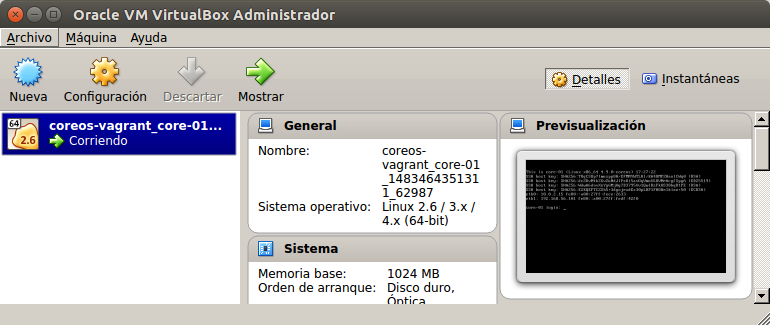
\includegraphics[width=0.8\textwidth]{images/figures/vboxcore01.png}
\caption{Máquina virtual \kode{core-01} desde VirtualBox.\label{fig:figure_placement_example}}
\end{figure}

El fichero \kode{Vagrantfile} establece el tamaño del clúster CoreOS que ha de ser creado por Vagrant. En este caso una sola instancia. Además, señala el parámetro \textit{discovery token}, utilizado para la detección del tamaño del clúster, valor que se reemplaza automáticamente cuando se inicia el desplique o levantamiento de una máquina, \kode{vagrant up}.

El fichero \kode{user-data} es el archivo de configuración \kode{cloud-config} que especifica el \kode{discovery token}, las variables de entorno y la lista de unidades de servicio que se deben iniciar de forma predeterminada. Vagrant copia el archivo \kode{cloud-config} en \kode{/var/lib/coreos-vagrant/vagrantfile-user-data}, dentro de la máquina virtual. De esta manera \kode{coreos-cloudinit} lee \kode{vagrantfile-user-data} en cada incio y lo utiliza para crear y reproducir el archivo de datos del usuario, \kode{user-data}, de la máquina.

Por su parte el fichero \kode{config.rb} especifica el número de nodos CoreOS y proporciona una opción para generar automáticamente un \textit{discovery token}.

\subsection{Interpretación del fichero de configuración Cloud-Config}

Una vez que el entorno se ha comprobado y preparado para su uso se accede al fichero \kode{user-data} que contiene la lógica necesaria sobre los servicios \kode{etcd2}, \kode{fleet} y \kode{flannel}.

A efectos de CoreOS este fichero se denomina como \kode{cloud-config}. Los parámetros \kode{coreos.etcd}, \kode{coreos.fleet} y \kode{coreos.flannel} son traducidos a una unidad \kode{systemd} parcial actuando como un archivo de configuración \kode{etcd2}, \kode{fleet} y \kode{flannel}, respectivamente. 

Como el entorno de plataforma admite la función de plantilla de \kode{coreos-cloudinit}, es posible automatizar la configuración de \kode{etcd2} con los campos \kode{\$private\_ipv4} y \kode{\$public\_ipv4}. Al generar un \textit{discovery token} se establece el tamaño del clúster, ya que \kode{etcd2} lo utiliza para determinar si todos los miembros se han unido a él. Después de inicializarse, el clúster puede crecer o reducirse. Por su parte \kode{fleet} y \kode{flannel} usan variables de entorno en su configuración.

La siguiente sección de este fichero pertenece a las unidades de servicio, de las que ya se encuentran definidas \kode{etcd2.service}, \kode{fleet.service}, \kode{flanneld.service}, donde esta última especifica la red en CoreOS y \kode{docker-tcp.socket}, el cual permite que se pueda usar el servicio \kode{docker-service} dentro de cada máquina.

\begin{codelisting}
\label{code:cloud-config1}
\codecaption{Fichero \kode{user-data}. Cloud-Config. Servicios.}
%= lang:ruby
\begin{code}
#cloud-config

---
coreos:
  etcd2:
    advertise-client-urls: http://$public_ipv4:2379
    initial-advertise-peer-urls: http://$private_ipv4:2380
    listen-client-urls: http://0.0.0.0:2379,http://0.0.0.0:4001
    listen-peer-urls: http://$private_ipv4:2380,http://$private_ipv4:7001
    discovery: https://discovery.etcd.io/acd611cb07df434a400bbd7e36d793a0
  fleet:
    public-ip: "$public_ipv4"
  flannel:
    interface: "$public_ipv4"
  units:
  - name: etcd2.service
    command: start
  - name: fleet.service
    command: start
  - name: flanneld.service
    drop-ins:
    - name: 50-network-config.conf
      content: |
        [Service]
        ExecStartPre=/usr/bin/etcdctl set /coreos.com/network/config \
                     '{ "Network": "10.1.0.0/16" }'
    command: start
  - name: docker-tcp.socket
    command: start
    enable: true
    content: |
      [Unit]
      Description=Docker Socket for the API

      [Socket]
      ListenStream=2375
      Service=docker.service
      BindIPv6Only=both

      [Install]
      WantedBy=sockets.target
\end{code}
\end{codelisting}

\subsection{Configuración y despliegue manual de las unidades de servicio}

El primer paso consiste en permitir que exista almacenamiento NFS compartido entre la máquina local y la máquina virtual CoreOS, con la intención de poder pasar a esta última las unidades de servicio a implementar. Para ello es necesario descomentar la siguiente línea, dentro del fichero \kode{Vagrantfile}:

\begin{codelisting}
\label{code:vagrantfile2}
\codecaption{Fichero \kode{Vagrantfile}}
%= lang:ruby
\begin{code}
.
config.vm.synced_folder ".", "/home/core/share", id: "core", :nfs => true, \
:mount_options => ['nolock,vers=3,udp']
.
\end{code}
\end{codelisting}

Así como instalarlo en el sistema anfitrión:

%= lang:bash
\begin{code}
$ sudo apt install nfs-kernel-server
\end{code}

También será necesario instalar el adaptador NFS en el sistema anfitrión y cargar los cambios. Esto creará, dentro de la máquina virtual, el directorio \kode{share}, compartido con el sistema anfitrión:

%= lang:bash
\begin{code}
$ sudo apt-get install nfs-kernel-server -y
$ vagrant reload --provision
\end{code}

\subsubsection{Unidad volume-public.service}

La primera unidad de servicio a crear será el volumen Docker compartido entre todos los contenedores. Para ello se crea, localmente, la ruta \kode{etc/sysctl/volume-public.service}. En este fichero se configura el servicio \kode{volume-public.service}. 

El contenido del mismo especifica que comenzará después de que lo haga el servicio Docker, el cual es requerido para el correcto funcionamiento. El servicio empezará directamente sin tiempo de espera. Una vez hecho se creará el volumen, añadiendo un enlace simbólico al mismo para todos los usuarios de la máquina. 

\begin{codelisting}
\label{code:volume-public.service}
\codecaption{Fichero \kode{etc/sysctl/volume-public.service}.}
%= lang:ruby
\begin{code}
[Unit] 
  Description= volume-public share between some-postgres, app-job, app-task and 
               some-nginx 
  After=docker.service
  Requires=docker.service

[Service] 
  TimeoutStartSec=0 
  ExecStart=/usr/bin/docker volume create --name volume-public

[Install] 
  WantedBy=multi-user.target
\end{code}
\end{codelisting}

\subsubsection{Unidad postgresql.service}

El siguiente paso consiste en agregar la unidades de servicio correspondiente a la base de datos de la aplicación. Para ello  se crea la ruta \kode{etc/sysctl/postgresql.service}. En este fichero se configura el servicio \kode{postgresql.service}.

El contenido del mismo especifica que comenzará después de que lo haga el servicio Docker y volume-public, requeridos para el correcto funcionamiento. El servicio empezará directamente sin tiempo de espera y se le indica el fichero donde ha de leer las variables de entorno necesarias. Si este servicio ya se ha ejecutado con anterioridad se procederá terminándolo y borrando el contenedor. Seguidamente, se comprobará, si ya existe la imagen del contenedor en la máquina, que sea la última versión disponible, de no ser así se obtendrá de nuevo. Llegado este punto la unidad de servicio comenzará creando el contenedor como se ha hecho hasta ahora, especificando la opción ha realizar si dicho contenedor quiere pararse. Además se añade un enlace simbólico al mismo para todos los usuarios de la máquina. 

\begin{codelisting}
\label{code:postgresql.service}
\codecaption{Fichero \kode{etc/sysctl/postgresql.service}.}
%= lang:ruby
\begin{code}
[Unit] 
  Description=PostgreSQL database 
  After=docker.service volume-public.service
  Requires=docker.service volume-public.service

[Service] 
  TimeoutStartSec=0
  EnvironmentFile=/home/core/share/etc/sysctl/fleet_machines.env
  ExecStartPre=-/usr/bin/docker kill some-postgres 
  ExecStartPre=-/usr/bin/docker rm some-postgres 
  ExecStartPre=/usr/bin/docker pull postgres 
  ExecStart=/usr/bin/docker run --rm --name some-postgres \
  -e "POSTGRES_USER=${POSTGRES_USER}" \
  -e "POSTGRES_PASSWORD=${POSTGRES_PASSWORD}" \
  -v "volume-public:/var/lib/posgresql" -p "5432:5432" postgres 
  ExecStop=/usr/bin/docker stop some-postgres 

[Install] 
  WantedBy=multi-user.target
\end{code}
\end{codelisting}

El contenido del fichero que especifica las variables de entorno hace referencia a las credenciales de la base de datos. Esto es controlado por el servicio fleet para todos aquellos procesos en ejecución.

\begin{codelisting}
\label{code:credentials}
\codecaption{Contenido del fichero \kode{fleet\_machines.env}}
\begin{code}
POSTGRES_USER=postgres
POSTGRES_PASSWORD=postgres
\end{code}
\end{codelisting}

\subsubsection{Unidad app-job.service}

La siguiente unidad de servicio será el contenedor ejecutable de la aplicación que crea, migra y alimenta la base de datos. Para ello se crea la ruta \kode{etc/sysctl/app-job.service}. En este fichero se configura el servicio \kode{app-job.service}.

El contenido del mismo especifica que comenzará después de que lo haga el servicio Docker, volume-public y postgresql, requeridos para el correcto funcionamiento. El servicio empezará directamente sin tiempo de espera, indicándole el fichero donde ha de leer las variables de entorno necesarias. Si este servicio ya se ha ejecutado con anterioridad se procederá terminándolo y borrando el contenedor. Seguidamente, se comprobará, si ya existe la imagen del contenedor en la máquina, que sea la última versión disponible, de no ser así se obtendrá de nuevo. Llegado este punto la unidad de servicio comenzará creando el contenedor como se ha hecho hasta ahora, especificando la opción ha realizar si dicho contenedor quiere pararse. Además se añade un enlace simbólico al mismo para todos los usuarios de la máquina. 

\begin{codelisting}
\label{code:app-job.service}
\codecaption{Fichero \kode{etc/sysctl/app-job.service}.}
%= lang:ruby
\begin{code}
[Unit] 
  Description=executable app-job container that creates, migrates, seeds and 
              populates the database
  After=docker.service volume-public.service postgresql.service
  Requires=docker.service volume-public.service postgresql.service

[Service] 
  TimeoutStartSec=0 
  EnvironmentFile=/home/core/share/etc/sysctl/fleet_machines.env
  ExecStartPre=-/usr/bin/docker kill app-job 
  ExecStartPre=-/usr/bin/docker rm app-job 
  ExecStartPre=/usr/bin/docker pull carolina/sample_app_rails_4_image:latest 
  ExecStart=/usr/bin/docker run --rm --name app-job \
  -v "volume-public:/usr/src/app/public" --entrypoint "/setup.sh" \
  -e "POSTGRES_USER=${POSTGRES_USER}" \
  -e "POSTGRES_PASSWORD=${POSTGRES_PASSWORD}" \
  -w "/usr/src/app" --link "some-postgres:db" \
  carolina/sample_app_rails_4_image:latest

[Install] 
  WantedBy=multi-user.target
\end{code}
\end{codelisting}

\subsubsection{Unidad app-task.service}

La siguiente unidad de servicio será el contenedor de la aplicación que ejecuta el servidor puma. Para ello se crea la ruta \kode{etc/sysctl/app-task.service}. En este fichero se configura el servicio \kode{app-task.service}.

El contenido del mismo especifica que comenzará después de que lo haga el servicio Docker, volume-public, postgresql y app-job, requeridos para el correcto funcionamiento. El servicio empezará directamente sin tiempo de espera, indicándole el fichero donde ha de leer las variables de entorno necesarias. Si este servicio ya se ha ejecutado con anterioridad se procederá terminándolo y borrando el contenedor. Seguidamente, se comprobará, si ya existe la imagen del contenedor en la máquina, que sea la última versión disponible, de no ser así se obtendrá de nuevo. Llegado este punto la unidad de servicio comenzará creando el contenedor como se ha hecho hasta ahora, especificando la opción ha realizar si dicho contenedor quiere pararse. Además se añade un enlace simbólico al mismo para todos los usuarios de la máquina. 

\begin{codelisting}
\label{code:app-task.service}
\codecaption{Fichero \kode{etc/sysctl/app-task.service}.}
%= lang:ruby
\begin{code}
[Unit] 
  Description=app-task container that runs the server puma
  After=docker.service volume-public.service postgresql.service app-job.service
  Requires=docker.service volume-public.service postgresql.service app-job.service

[Service] 
  TimeoutStartSec=0 
  EnvironmentFile=/home/core/share/etc/sysctl/fleet_machines.env
  ExecStartPre=-/usr/bin/docker kill app-task 
  ExecStartPre=-/usr/bin/docker rm app-task
  ExecStartPre=/usr/bin/docker pull carolina/sample_app_rails_4_image:latest 
  ExecStart=/usr/bin/docker run --rm --name app-task \
  -e "POSTGRES_USER=${POSTGRES_USER}" \
  -e "POSTGRES_PASSWORD=${POSTGRES_PASSWORD}" \
  -w "/usr/src/app" -v "volume-public:/usr/src/app/public" \
  --link "some-postgres:db" carolina/sample_app_rails_4_image:latest \
  /bin/bash -c "cp config/database.yml.postgresql config/database.yml \
  && puma -p 9292"
  ExecStop=/usr/bin/docker stop app-task

[Install] 
  WantedBy=multi-user.target
\end{code}
\end{codelisting}

\subsubsection{Unidad nginx.service}

La siguiente unidad del servicio será el contenedor que ejecuta el servidor nginx. Para ello se crea la ruta \kode{etc/sysctl/nginx.service}. En este fichero se configura el servicio \kode{nginx.service}.

El contenido del mismo especifica que comenzará después de que lo haga el servicio Docker, volume-public, postgresql, app-job y app-task, requeridos para el correcto funcionamiento. El servicio empezará directamente sin tiempo de espera. Si este servicio ya se ha ejecutado con anterioridad se procederá terminándolo y borrando el contenedor. Seguidamente, se comprobará, si ya existe la imagen del contenedor en la máquina, que sea la última versión disponible, de no ser así se obtendrá de nuevo. Llegado este punto la unidad de servicio comenzará creando el contenedor como se ha hecho hasta ahora, teniendo en cuenta que ahora la redirección de puertos se ha establecido para trabajar el puerto 80 de la máquina CoreOS con el puerto 80 de la aplicación, especificando la opción ha realizar si dicho contenedor quiere pararse. Además se añade un enlace simbólico al mismo para todos los usuarios de la máquina. 

\begin{codelisting}
\label{code:nginx.service}
\codecaption{Fichero \kode{etc/sysctl/nginx.service}.}
%= lang:ruby
\begin{code}
[Unit] 
  Description=some-nginx container that runs a reverse proxy server and a 
              web server
  After=docker.service volume-public.service postgresql.service app-job.service 
        app-task.service
  Requires=docker.service volume-public.service postgresql.service 
           app-job.service app-task.service

[Service] 
  TimeoutStartSec=0 
  ExecStartPre=-/usr/bin/docker kill some-nginx 
  ExecStartPre=-/usr/bin/docker rm some-nginx
  ExecStartPre=/usr/bin/docker pull nginx 
  ExecStart=/usr/bin/docker run --rm --name some-nginx \
  -v "/home/core/share/etc/sysctl/nginx.conf:/etc/nginx/conf.d/default.conf" \
  -p "80:80" --link "app-task:app" -v "volume-public:/usr/src/app/public" nginx 
  ExecStop=/usr/bin/docker stop some-nginx

[Install] 
  WantedBy=multi-user.target
\end{code}
\end{codelisting}

\subsubsection{Despliegue manual}

Una vez que ya se han configurado y escrito las 5 unidades de servicio necesarias el siguiente paso es preparar su despliegue. Para el reconocimiento de las unidades éstas tienen que ubicarse bajo el servicio \kode{systemd}. Por ello el primer paso será la copia de las mismas al directorio \kode{/etc/systemd/system/}. El funcionamiento de las unidades pasa por dos estados. El primer estado es la habilitación del servicio, esto creará el enlace simbólico de la unidad para todos los usuarios. El segundo estado es el comienzo del mismo.

Dicho esto, se crea un script denominado \kode{coreos-service-units-deploy.sh}, con permisos \kode{chmod +x}, que se encargará de realizar la copia de las unidades bajo \kode{systemd} y que habilitará y comenzará los servicios.

\begin{codelisting}
\label{code:coreos-service-units-deploy}
\codecaption{Fichero \kode{coreos-service-units-deploy.sh}.}
%= lang:bash
\begin{code}
#!/bin/bash

sudo cp share/etc/sysctl/* /etc/systemd/system/

sudo systemctl enable volume-public.service
sudo systemctl enable postgresql.service
sudo systemctl enable app-job.service
sudo systemctl enable app-task.service
sudo systemctl enable nginx.service

sudo systemctl start volume-public.service
sudo systemctl start postgresql.service
sudo systemctl start app-job.service
sudo systemctl start app-task.service
sudo systemctl start nginx.service
\end{code}
\end{codelisting}

Con la intención de que este script se ejecute al iniciar la máquina CoreOS se añade al fichero \kode{Vagrantfile} una línea que indicará la ruta del mismo para hacer uso del fichero y provisionar la máquina con las directivas incluidas en él.

\begin{codelisting}
\label{code:vagrantfile3}
\codecaption{Fichero \kode{Vagrantfile}}
%= lang:ruby
\begin{code}
.
config.vm.provision "shell", path: "coreos-service-units-deploy.sh"
.
\end{code}
\end{codelisting}

Finalmente los pasos necesarios para iniciar la máquina serán la recarga de la misma con la opción de provisión, tanto por el hecho de que la máquina pueda encontrarse ya iniciada y por si se han hecho cambios en los ficheros que influyen en la construcción de los servicios internos a llevar a cabo. Además, habrá que acceder a dicha máquina. Así se crea un segundo script llamado \kode{coreos-deploy.sh}, con permisos \kode{chmod +x}, que se ejecutará de ahora en adelante para tal propósito.

\begin{codelisting}
\label{code:vagrantfile2}
\codecaption{Fichero \kode{coreos-deploy.sh}.}
%= lang:bash
\begin{code}
#!/bin/bash

vagrant reload --provision
vagrant ssh core-01
\end{code}
\end{codelisting}

Si se inicia el despliegue manual se comprueba el correcto funcionamiento de la aplicación, donde todos los servicios estarán en estado activo o cargado:

%= lang:bash
\begin{code}
$ ./coreos-deploy.sh
\end{code}

\begin{figure}[H]
\centering
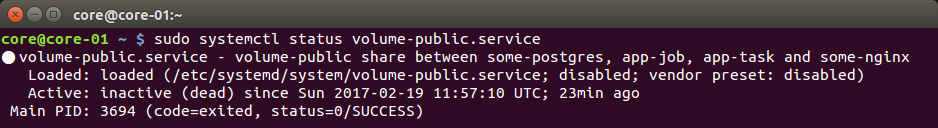
\includegraphics[width=0.9\textwidth]{images/figures/volume-public.service.png}
\caption{Estado de la unidad \kode{volume-public.service}.\label{fig:figure_placement_example}}
\end{figure}

\begin{figure}[H]
\centering
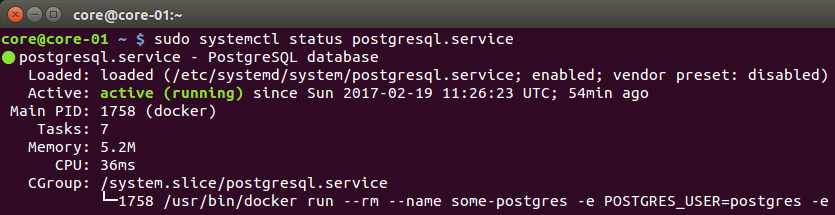
\includegraphics[width=0.9\textwidth]{images/figures/postgresql.service.png}
\caption{Estado de la unidad \kode{postgresql.service}..\label{fig:figure_placement_example}}
\end{figure}

\begin{figure}[H]
\centering
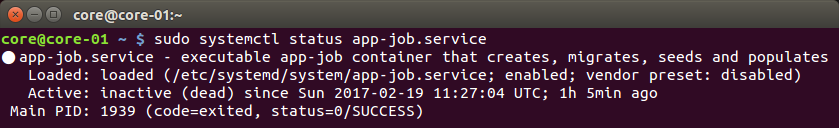
\includegraphics[width=0.9\textwidth]{images/figures/app-job.service.png}
\caption{Estado de la unidad \kode{app-job.service}.\label{fig:figure_placement_example}}
\end{figure}

\begin{figure}[H]
\centering
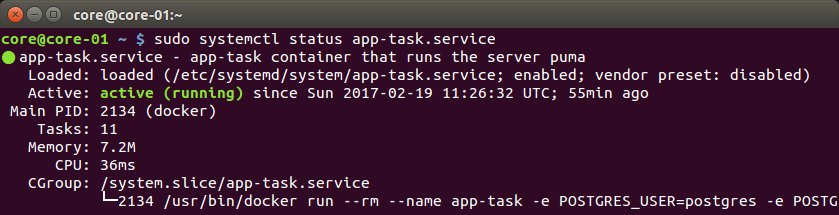
\includegraphics[width=0.9\textwidth]{images/figures/app-task.service.png}
\caption{Estado de la unidad \kode{app-task.service}.\label{fig:figure_placement_example}}
\end{figure}

\begin{figure}[H]
\centering
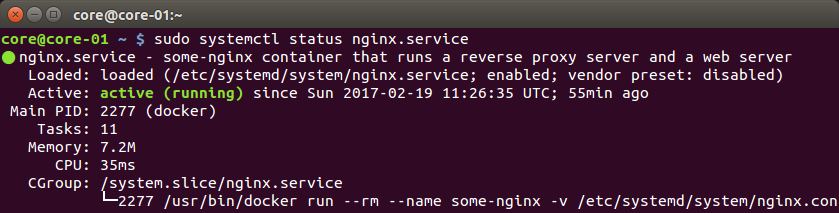
\includegraphics[width=0.9\textwidth]{images/figures/nginx.service.png}
\caption{Estado de la unidad \kode{nginx.service}.\label{fig:figure_placement_example}}
\end{figure}

Por último se accede a la aplicación en modo consola desde la máquina CoreOS y en modo gráfico desde el sistema anfitrión:

\begin{figure}[H]
\centering
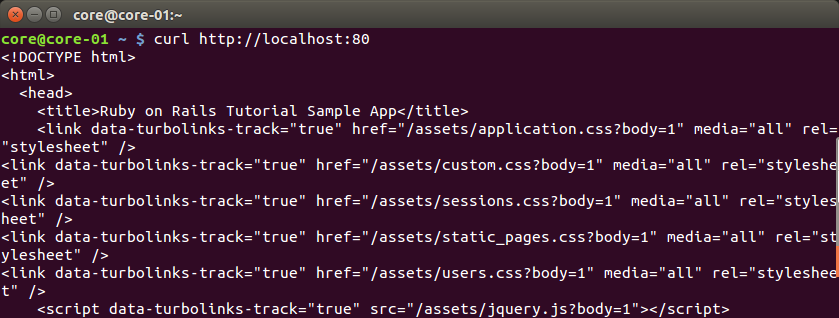
\includegraphics[width=0.9\textwidth]{images/figures/coreosmanualcurl.png}
\caption{Acceso a la aplicación desde la máquina CoreOS.\label{fig:figure_placement_example}}
\end{figure}

\begin{figure}[H]
\centering
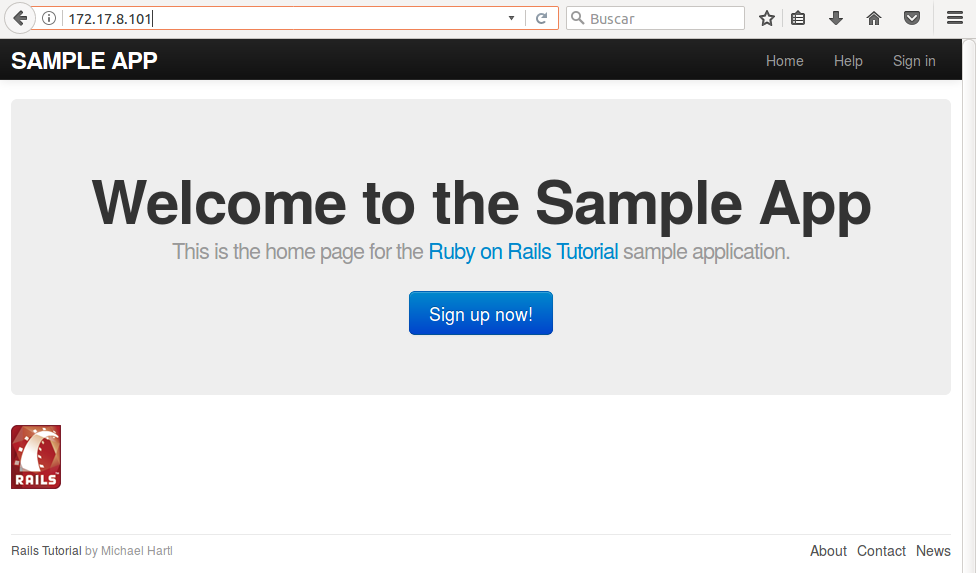
\includegraphics[width=0.9\textwidth]{images/figures/coreosmanualhost.png}
\caption{Acceso a la aplicación desde el sistema anfitrión.\label{fig:figure_placement_example}}
\end{figure}

\subsection{Configuración y despliegue automático de las unidades de servicio}

El despliegue ideal de la aplicación a través de las unidades de servicio que la componen sería de manera automática. Esto se implementa en CoreOS a partir del fichero denominado \kode{cloud-config} que se corresponde con \kode{user-data}. Este fichero especifica el orden de las unidades ha desplegar y las acciones de habilitación y comienzo de los servicios a los que hacen referencia.

Esta vez no se usará el almacenamiento NFS compartido así que el fichero con las variables de entorno también es descrito, índicandole la nueva ruta en la que se encuentra, sus permisos y contenido. 

Así, la confección de este fichero queda de la siguiente manera:

\begin{codelisting}
\label{code:vagrantfile2}
\codecaption{Fichero \kode{user-data}.}
%= lang:ruby
\begin{code}
#cloud-config

---
write_files:
  - path: "/etc/fleet_machines.env"
    permissions: "0644"
    content: |
      POSTGRES_USER=postgres
      POSTGRES_PASSWORD=postgres
coreos:
  etcd2:
    advertise-client-urls: http://$public_ipv4:2379
    initial-advertise-peer-urls: http://$private_ipv4:2380
    listen-client-urls: http://0.0.0.0:2379,http://0.0.0.0:4001
    listen-peer-urls: http://$private_ipv4:2380,http://$private_ipv4:7001
    discovery: https://discovery.etcd.io/e26b5e212eaa7df4a003cee8bac6ed16
  fleet:
    public-ip: "$public_ipv4"
  flannel:
    interface: "$public_ipv4"
  units:
  - name: etcd2.service
    command: start
  - name: fleet.service
    command: start
  - name: flanneld.service
    drop-ins:
    - name: 50-network-config.conf
      content: |
        [Service]
        ExecStartPre=/usr/bin/etcdctl set /coreos.com/network/config '{ "Network": "10.1.0.0/16" }'
    command: start
  - name: docker-tcp.socket
    command: start
    enable: true
    content: |
      [Unit]
      Description=Docker Socket for the API

      [Socket]
      ListenStream=2375
      Service=docker.service
      BindIPv6Only=both

      [Install]
      WantedBy=sockets.target
  - name: volume-public.service
    command: start
    enable: true
    content: |
      [Unit] 
      Description= volume-public share between some-postgres, app-job, app-task and some-nginx 
      After=docker.service
      Requires=docker.service

      [Service] 
      TimeoutStartSec=0 
      ExecStart=/usr/bin/docker volume create --name volume-public

      [Install] 
      WantedBy=multi-user.target
  - name: postgresql.service
    command: start
    enable: true
    content: |
      [Unit] 
      Description=PostgreSQL database 
      After=docker.service volume-public.service
      Requires=docker.service volume-public.service

      [Service] 
      TimeoutStartSec=0
      EnvironmentFile=/etc/fleet_machines.env
      ExecStartPre=-/usr/bin/docker kill some-postgres 
      ExecStartPre=-/usr/bin/docker rm some-postgres 
      ExecStartPre=/usr/bin/docker pull postgres 
      ExecStart=/usr/bin/docker run --rm --name some-postgres \
      -e "POSTGRES_USER=${POSTGRES_USER}" -e "POSTGRES_PASSWORD=${POSTGRES_PASSWORD}" \
      -v "volume-public:/var/lib/posgresql" -p "5432:5432" postgres 
      ExecStop=/usr/bin/docker stop some-postgres

      [Install] 
      WantedBy=multi-user.target
  - name: app-job.service
    command: start
    enable: true
    content: |
      [Unit] 
      Description=executable app-job container that creates, migrates, seeds and populates the database
      After=docker.service volume-public.service postgresql.service
      Requires=docker.service volume-public.service postgresql.service

      [Service] 
      TimeoutStartSec=0 
      EnvironmentFile=/etc/fleet_machines.env
      ExecStartPre=-/usr/bin/docker kill app-job 
      ExecStartPre=-/usr/bin/docker rm app-job 
      ExecStartPre=/usr/bin/docker pull carolina/sample_app_rails_4_image:latest 
      ExecStart=/usr/bin/docker run --rm --name app-job -v "volume-public:/usr/src/app/public" --entrypoint "/setup.sh" \
      -e "POSTGRES_USER=${POSTGRES_USER}" -e "POSTGRES_PASSWORD=${POSTGRES_PASSWORD}" \
      -w "/usr/src/app" --link "some-postgres:db" \
      carolina/sample_app_rails_4_image:latest

      [Install] 
      WantedBy=multi-user.target
  - name: app-task.service
    command: start
    enable: true
    content: |
      [Unit] 
      Description=app-task container that runs the server puma
      After=docker.service volume-public.service postgresql.service app-job.service
      Requires=docker.service volume-public.service postgresql.service app-job.service

      [Service] 
      TimeoutStartSec=0 
      EnvironmentFile=/etc/fleet_machines.env
      ExecStartPre=-/usr/bin/docker kill app-task 
      ExecStartPre=-/usr/bin/docker rm app-task
      ExecStartPre=/usr/bin/docker pull carolina/sample_app_rails_4_image:latest 
      ExecStart=/usr/bin/docker run --rm --name app-task \
      -e "POSTGRES_USER=${POSTGRES_USER}" -e "POSTGRES_PASSWORD=${POSTGRES_PASSWORD}" \
      -w "/usr/src/app" -v "volume-public:/usr/src/app/public" --link "some-postgres:db" \
      carolina/sample_app_rails_4_image:latest \
      /bin/bash -c "cp config/database.yml.postgresql config/database.yml && puma -p 9292"
      ExecStop=/usr/bin/docker stop app-task

      [Install] 
      WantedBy=multi-user.target
  - name: nginx.service
    command: start
    enable: true
    content: |
      [Unit] 
      Description=some-nginx container that runs a reverse proxy server and a web server
      After=docker.service volume-public.service postgresql.service app-job.service app-task.service
      Requires=docker.service volume-public.service postgresql.service app-job.service app-task.service

      [Service] 
      TimeoutStartSec=0 
      ExecStartPre=-/usr/bin/docker kill some-nginx 
      ExecStartPre=-/usr/bin/docker rm some-nginx
      ExecStartPre=/usr/bin/docker pull nginx 
      ExecStart=/usr/bin/docker run --rm --name some-nginx \
      -v "/home/coreos/share/etc/sysctl/nginx.conf:/etc/nginx/conf.d/default.conf" \
      -p "80:80" --link "app-task:app" -v "volume-public:/usr/src/app/public" nginx 
      ExecStop=/usr/bin/docker stop some-nginx

      [Install] 
      WantedBy=multi-user.target
  \end{code}
\end{codelisting}

Como se puede apreciar, ya no es necesaría la copia de los ficheros de las unidades del entorno local a la máquina CoreOS. Ahora simplemente se hace uso de estos ficheros y de los correspondientes a \kode{/fleet\_machines.env} y \kode{nginx.conf} desde el directorio compartido. Por lo tanto ya no es necesaria la línea de provisión del script en el fichero \kode{Vagranfile}

Si se inicia el despliegue manual:

%= lang:bash
\begin{code}
$ ./coreos-deploy.sh
\end{code}

se comprueba el correcto funcionamiento de la aplicación, nuevamente.

\subsection{Resultado}

\section{Iteración 5: Despliegue multimáquina con unidades usando CoreOS}

